\documentclass[conference]{sig-alternate}
%\documentclass{acm_proc_article-sp}

\makeatletter
\newif\if@restonecol

\let\algorithm\relax
\let\endalgorithm\relax
\usepackage[tight,footnotesize]{subfigure}
\usepackage {paralist}
\usepackage{comment}
\usepackage{array}
\usepackage{amsmath}
\usepackage{graphicx}
\usepackage{amssymb}
\usepackage{cite}
\usepackage{url}
\makeatother
\makeatletter
\providecommand{\tabularnewline}{\\}


\newtheorem{clm}{Claim}
\begin{document}

\title{Real-Time Length-based Contention Management for STM}


%\author{Mohammed Elshambakey
%\affil{ECE Dept., Virginia Tech, Blacksburg, VA 24060, USA}
%Binoy Ravindran
%\affil{ECE Dept., Virginia Tech, Blacksburg, VA 24060, USA}
%}

\begin{comment}
\author{\IEEEauthorblockN{Mohammed Elshambakey}
\IEEEauthorblockA{ECE Dept, Virginia Tech\\
Blacksburg, VA 24061, USA\\
Email: shambake@vt.edu}
\and
\IEEEauthorblockN{Binoy Ravindran}
\IEEEauthorblockA{ECE Dept, Virginia Tech\\
Blacksburg, VA 24061, USA\\
Email: binoy@vt.edu}
}
\end{comment}


\maketitle

\begin{abstract}
We consider software transactional memory (STM) concurrency control for multicore real-time software, and present a novel contention manager (CM) for resolving transactional conflicts, called length-based CM (or LCM). We upper bound transactional retries and response times under LCM, when used with G-EDF and  G-RMA schedulers. We identify the conditions under which LCM is superior to previous real-time CMs, and show how LCM can achieve higher schedulability than retry-loop lock-free synchronization for G-EDF systems. %We show that, LCM achieves higher schedulability for larger  atomic section lengths than that with past CMs.
Presented work is analytical as the questions we try to answer are analytical, so our results. Experimental evaluation will be done in future work.
\end{abstract}

%\maketitle

\section{Introduction}
\label{sec:intro}

Lock-based concurrency control suffers from programmability, scalability, and composability challenges~\cite{Herlihy:2006:AMP:1146381.1146382}. These challenges are exacerbated in emerging multicore architectures, on which improved software performance must be achieved by exposing greater concurrency.  Transactional memory (TM) is an alternative synchronization model for shared memory data objects that promises to alleviate these difficulties.  With TM, programmers organize code that read/write shared objects as transactions, which appear to execute atomically. Two transactions conflict if they access the same object and one access is a write. When that happens, a contention manager (or CM)
%~\cite{Guerraoui:2005:TTT:1073814.1073863} 
resolves the conflict by aborting one and allowing the other to commit, yielding (the illusion of) atomicity. Aborted transactions are re-started.
%often immediately.  
In addition to a simple programming model, TM provides performance comparable to highly concurrent fine-grained locking and lock-free approaches,  
%~\cite{Saha:2006:MHP:1122971.1123001}, 
and is composable. 
%~\cite{Harris:2005:CMT:1065944.1065952}. 
TM has been proposed in hardware, called HTM,  
%(e.g.,~\cite{austenmc:tcc:dissertation:2009}), 
and in software, called STM,  
%(e.g.,~\cite{sha95}),  
with the usual tradeoffs: HTM has lesser overhead, but needs transactional support in hardware; STM is available on any hardware. See~\cite{tm-book10} for an excellent overview on TM.


Given STM's programmability, scalability, and composability advantages, we consider it for concurrency control in multicore real-time software. Doing so requires bounding transactional  retries, as real-time threads, which subsume transactions, must satisfy time constraints.  Retry bounds in STM are dependent on the CM policy at hand. Thus, real-time CM is logical.

Past research on real-time CM have proposed resolving transactional contention using dynamic and fixed priorities of parent threads, resulting in Earliest-Deadline-First-based CM (ECM) and Rate Monotonic Assignment-based CM (RCM), respectively~\cite{fahmy2009bounding,fahmy2009response,stmconcurrencycontrol:emsoft11}.
These works show that, ECM and RCM, when used with Global EDF (G-EDF) and Global RMA  (G-RMA) schedulers, respectively, achieve higher schedulability than locking and lock-free synchronization techniques only under some ranges for the maximum atomic section length. This raises a fundamental question: is it possible to increase the atomic section length by an alternative CM design, so that STM's schedulability advantage has a larger coverage? 

We answer this question by designing a novel CM that can be used with both dynamic and fixed priority (global) multicore real-time schedulers: length-based CM or LCM (Section~\ref{sec 9.1}). LCM resolves conflicts based on the priority of conflicting jobs, besides the length of the interfering atomic section, and the length of the interfered atomic section.  We establish LCM's retry and response time upper bounds, when used with G-EDF (Section~\ref{response g-edf/lcm}) and with G-RMA (Section~\ref{rma}) schedulers. We identify the conditions under which G-EDF/LCM outperforms ECM (Section~\ref{performance g-edf-lcm}), lock-free apporach (Section~\ref{gedf-lcm-lock-free}) and G-RMA/LCM outperforms RCM (Section~\ref{rma eval}). 

\section{Related Work}
\label{sec:past}

Transactional-like concurrency control without using locks, for real-time systems, has been previously studied in the context of non-blocking data structures (e.g.,~\cite{anderson95realtime}). Despite their numerous advantages over locks 
(e.g., deadlock-freedom), 
their programmability has remained a challenge. 
Past studies show that they are best suited for simple data structures where their retry cost is competitive to the cost of lock-based synchronization~\cite{bc+08}.  In contrast, STM is semantically simpler~\cite{Herlihy:2006:AMP:1146381.1146382}, and is often the only viable lock-free solution for complex data structures (e.g., red/black tree)~\cite{key-1} and nested critical sections~\cite{Saha:2006:MHP:1122971.1123001}.

STM concurrency control for real-time systems has been previously studied in~\cite{manson2006preemptible,fahmy2009bounding,sarni2009real,schoeberl2010rttm,key-1,barrosmanaging,stmconcurrencycontrol:emsoft11}.


\cite{manson2006preemptible} proposes a restricted version of STM for uniprocessors. Uniprocessors do not need contention management.

\cite{fahmy2009bounding} bounds response times in distributed multiprocessor systems with STM synchronization. They consider Pfair scheduling, limit to small atomic regions with fixed size, and limit transaction execution to span at most two quanta. In contrast, we allow transaction lengths 
with  arbitrary duration. 

\cite{sarni2009real} presents real-time scheduling of transactions and serializes transactions based on deadlines. However, the work does not bound retries and response times. In contrast, we establish such bounds.


\cite{schoeberl2010rttm} proposes real-time HTM. The work does not describe how transactional conflicts are resolved. Besides, the retry bound assumes that the worst case conflict between atomic sections of different tasks occurs when the sections are released at the same time. However, we show that this is not the worst case. We develop retry and response time upper bounds based on much worse conditions.


\cite{key-1} upper bounds retries and response times for  ECM with G-EDF, and identify the tradeoffs against locking and lock-free protocols. Similar to~\cite{schoeberl2010rttm},~\cite{key-1} also assumes that the worst case conflict between atomic sections occurs when the sections are released simultaneously. 

The ideas in~\cite{key-1} are extended in~\cite{barrosmanaging}, which presents three real time CM designs. But no retry bounds nor schedulability analysis techniques are presented for those CMs. 

\cite{stmconcurrencycontrol:emsoft11} presents the ECM and RCM contention managers, and upper bounds transactional retries and response times under them. The work also identifies the conditions under which ECM and RCM are superior to locking and lock-free techniques. In particular, they show that, the STM superiority holds only under some ranges for the maximum atomic section length. Our work builds upon this result.

\section{Preliminaries}
\label{sec:model}

We consider a multiprocessor system with $m$ identical processors and $n$ sporadic tasks $\tau_1, \tau_2,\ldots, \tau_n$. The $k^{th}$ instance (or job) of a task $\tau_i$ is denoted $\tau_i^k$. Each task $\tau_i$ is specified by its worst case execution time (WCET) $c_i$, its minimum period $T_i$ between any two consecutive instances, and its relative deadline $D_i$, where $D_i=T_i$. Job $\tau_i^j$ is released at time $r_i^j$ and must finish no later than its absolute deadline $d_i^j=r_i^j+D_i$. Under a fixed priority scheduler such as G-RMA, $p_i$ determines $\tau_i$'s (fixed) priority and it is constant for all instances of $\tau_i$. Under a dynamic priority scheduler such as G-EDF, a $\tau_i^j$'s priority, $p_i^j$, differs from  instance to another. 
A task $\tau_j$ may interfere with task $\tau_i$ for a number of times during an interval $L$, and this number is denoted as $G_{ij}(L)$. 
$\tau_j$'s workload that interferes with $\tau_i$ during $L$ is denoted $W_{ij}(L)$.


\textit{Shared objects.} A task may need to access (i.e., read, write) shared, in-memory objects while it is executing any of its atomic sections, which are synchronized using STM. 
The set of atomic sections of task $\tau_i$ is denoted $s_i$. $s_i^k$ is the $k^{th}$ atomic section of $\tau_i$. 
Each object, $\theta$, can be accessed by multiple tasks. The set of objects accessed by $\tau_i$ is $\theta_i$ without repeating objects.
The set of atomic sections used by $\tau_i$ to access $\theta$ is $s_i(\theta)$, and the sum of the lengths of those atomic sections is $len(s_i(\theta))$. $s_i^k(\theta)$ is the $k^{th}$ atomic section of $\tau_i$ that accesses $\theta$. $s_i^k(\theta)$  executes for a duration $len(s_i^k(\theta))$.
% which is the whole length of the atomic section (and not just the part that accesses $\theta$). 
%Thus, for two objects $\theta_1$ and $\theta_2$ that are accessed within the same atomic section of $T_i$, $len(s_i^k(\theta1))=len(s_i^k(\theta2))$. 
%If $\theta$ is shared by multiple tasks, then $s(\theta)$ is the set of atomic sections of all tasks accessing $\theta$, and 
The set of tasks sharing $\theta$ with $\tau_i$ is denoted $\gamma_i(\theta)$. Atomic sections are non-nested, and each atomic section is assumed to access only one object to be consistent with the assumptions made in~\cite{stmconcurrencycontrol:emsoft11}.% that enabled comparison with retry-loop lock-free approach \cite{key-5}.

The maximum-length atomic section in $\tau_i$ that accesses $\theta$ is denoted $s_{i_{max}} (\theta)$, while the maximum one among all tasks is $s_{max} (\theta)$, and the maximum (minimum) one among tasks with priorities lower than that of $\tau_i$ is $s_{max}^i (\theta)$ ($s_{min}^i (\theta)$).

\textit{STM retry cost.} If two or more atomic sections conflict, the CM will commit one section and abort and retry the others, increasing the time to execute the aborted sections. The increased time that an atomic section $s_i^p (\theta)$ will take to execute due to conflict with another section $s_j^k (\theta)$, is denoted $W_{i}^{p}(s_{j}^{k}(\theta))$. If an atomic section, $s_i^p$, is already executing, and another atomic section $s_j^k$ tries to access a shared object with $s_i^p$, then $s_j^k$ is said to "interfere" or "conflict" with $s_i^p$, and job of $s_j^k$ is the "interfering job", while job of $s_i^p$ is the "interfered job". The total time that a task $\tau_i$'s atomic sections have to retry over $T_i$ is denoted $RC(T_i)$.

\textit{LCM notations.} $\psi$ is a chosen threshold value. $\alpha$ is a percentage value. $\alpha_{ij}^{kl}$ is the $\alpha$ value corresponding to $\psi$ for interference of $s_i^k(\theta)$ by $s_j^l(\theta)$. $c_{ij}^{kl}$ is the result of $len(s_j^l(\theta))/len(s_i^k(\theta))$.

\section{Length-based Contention Manager (LCM)}

LCM resolves conflicts based on the priority of conflicting jobs, besides the length of the interfering atomic section, and the length of the interfered atomic section. So, its design is less straight forward than ECM and RCM~\cite{stmconcurrencycontrol:emsoft11} as they depend only on the priority of the conflicting jobs. This modification in design allows lower priority jobs, under LCM, to retry for less time than ECM and RCM, but higher priority jobs, sometimes, wait for lower priority ones with bounded priority-inversion.

\subsection{\label{sec 9.1} LCM: Design and Rationale}

For both ECM and RCM, $s_{i}^{k}(\theta)$ can be totally repeated if $s_{j}^{l}(\theta)$ --- which belongs to a higher priority job $\tau_{j}^b$ than $\tau_{i}^a$ --- conflicts with $s_{i}^{k}(\theta)$
at the end of its execution, while $s_{i}^{k}(\theta)$ is just about
to commit. Thus, LCM  uses the remaining length of $s_{i}^{k}(\theta)$ when it is interfered,
as well as $len(s_{j}^{l}(\theta))$, to decide which transaction must be aborted. If $s_i^k (\theta)$ is the one which interferes with $s_j^l (\theta)$, then $s_j^l (\theta)$ commits because it belongs to the higher priority job and it started before $s_i^k (\theta)$.

We assume that 
\begin{equation}
len(s_{j}^{l}(\theta))=c_{ij}^{kl}len(s_{i}^{k}(\theta))
\label{cm_eq}\end{equation}
where $c_{ij}^{kl}\in]0,\infty[$, to cover all possible lengths of $s_{j}^{l}(\theta)$.
Our idea is to reduce the opportunity for the abortion of $s_{i}^{k}(\theta)$ if it is close to committing when interfered, and $len(s_{j}^{l}(\theta))$ is large. This abortion opportunity is reduced more and more as $s_{i}^{k}(\theta)$ gets closer to its end of execution, or $len(s_{j}^{l}(\theta))$ gets larger. 

On the other side, as $s_{i}^{k}(\theta)$ is interfered early,
or $len(s_{j}^{l}(\theta))$ is small compared to $s_{i}^{k}(\theta)$'s remaining length, the abortion opportunity 
is increased even if $s_i^k (\theta)$ is close to its end of execution. To decide whether $s_{i}^{k}(\theta)$ should abort or not, we use a threshold value $\psi\in[0,1]$, that determines
the length percentage of $s_{i}^{k}(\theta)$ below which $s_{i}^{k}(\theta)$ will abort due to $s_{j}^{l}(\theta)$. This percentage value is denoted $\alpha_{ij}^{kl}$. 
%
If the percentage value is 0, it means not to abort, and 1 means to abort. 


%
\begin{figure}[htbp]
\centering
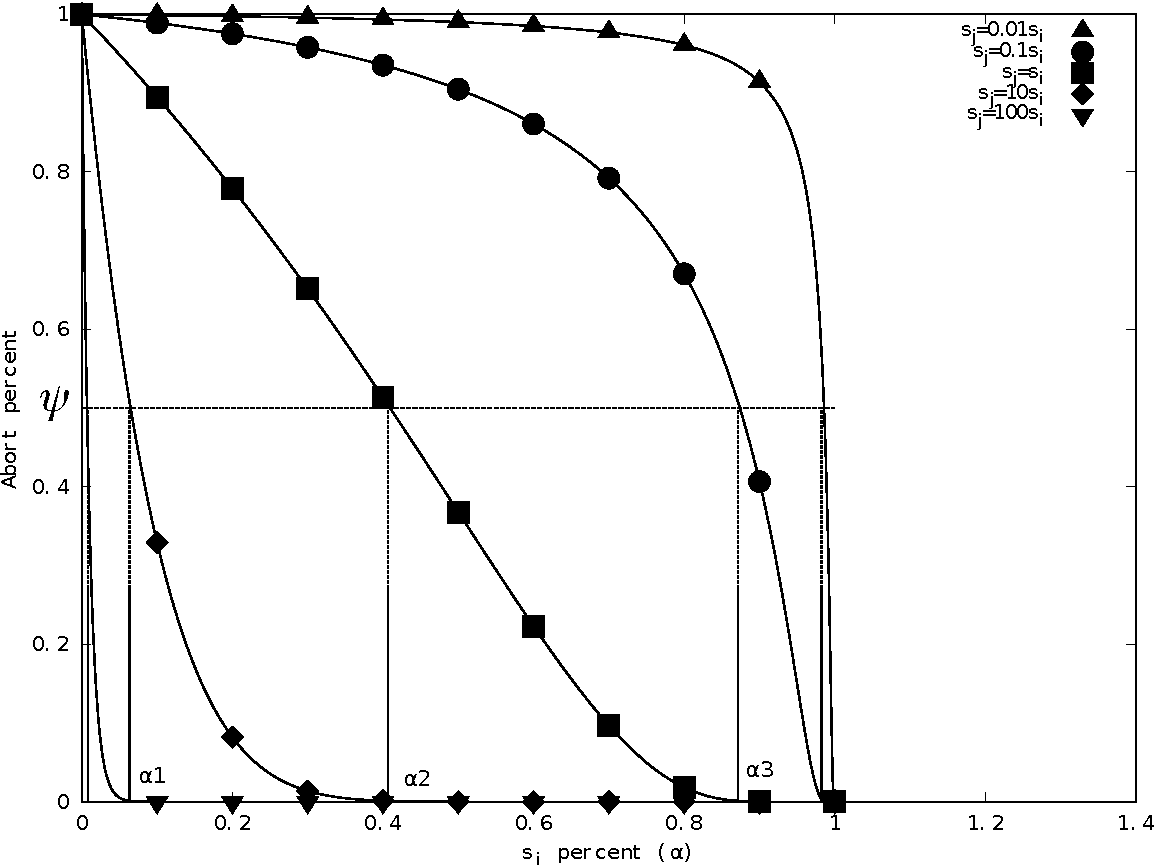
\includegraphics[scale=0.4]{figures/figure16}
\caption{\label{fig16}Interference of $s_{i}^{k}(\theta)$ by various lengths of 
$s_{j}^{l}(\theta)$}
\end{figure}

The behavior of LCM  is illustrated in Figure \ref{fig16}. The figure represents five different lengths of $s_{j}^{l}(\theta)$
interfering with $s_{i}^{k}(\theta)$ at all points of $s_{i}^{k}(\theta)$.
For a specific curve (which means a specific length for $s_{j}^{l}(\theta)$ with respect to $s_i^k(\theta)$),
$\psi$ determines the percentage of $len(s_{i}^{k}(\theta))$
below which $s_{i}^{k}(\theta)$ will be aborted. For example, for
$len(s_{j}^{l}(\theta))=0.1\times len(s_{i}^{k}(\theta))$, $s_{i}^{k}(\theta)$
will be aborted by $s_{j}^{l}(\theta)$ if the latter interferes with
$s_{i}^{k}(\theta)$ no later than $s_{i}^{k}(\theta)$ reaches $\alpha3$
percentage of its length ($\alpha3$ is shown in Figure~\ref{fig16}). After that, $s_{j}^{l}(\theta)$ will have
to retry. As $len(s_{j}^{l}(\theta))$ decreases, the opportunity
that it will abort $s_{i}^{k}(\theta)$ at a higher percentage $\alpha_{max}$
increases (as illustrated in Figure~\ref{fig16}, $\alpha3>\alpha2>\alpha1$ for reduced length of $s_j^l(\theta)$). The function that is used to represent the 
different curves in Figure \ref{fig16} is:
 \begin{equation}
f(c_{ij}^{kl},\alpha)=e^{\frac{-c_{ij}^{kl}\alpha}{1-\alpha}}\label{eq49}\end{equation}
where $c_{ij}^{kl}$ is calculated by~(\ref{cm_eq}), but $\alpha$ changes
along each curve, with a specific value of $\alpha$ corresponds to $\psi$. This function achieves the desired requirement that the abortion opportunity is reduced as $s_{i}^{k}(\theta)$ gets
closer to its end of execution (as $\alpha\rightarrow1,\, f(c_{ij}^{kl},1)\rightarrow0$),
or as the length of the conflicting transaction is large (as $c_{ij}^{kl}\rightarrow\infty,\, f(\infty,\alpha)\rightarrow0$).
Meanwhile, this abortion opportunity is increased as $s_{i}^{k}(\theta)$
is interfered closer to its release (as $\alpha\rightarrow0,\, f(c_{ij}^{kl},0)\rightarrow1$),
or as the length of the conflicting transaction decreases (as $c_{ij}^{kl}\rightarrow0,\, f(0,\alpha)\rightarrow1$).

As $s_{j}^{l}(\theta)$ belongs to a higher priority job than $s_{i}^{k}(\theta)$, if $s_{j}^{l}(\theta)$ starts before or at the same start time of
$s_{i}^{k}(\theta)$, then $s_{i}^{k}(\theta)$ will have to abort
and retry. But if $s_{j}^{l}(\theta)$
starts after $s_{i}^{k}(\theta)$, then the comparison illustrated
previously will be applied. LCM is not a central CMs, which means each two transactions have to decide which one of them is to commit.

\begin{clm}
\label{LCM_higher_rc}
Let $s_{j}^{l}(\theta)$ interfere with $s_{i}^{k}(\theta)$ at $\alpha_{ij}^{kl}$. Then, the maximum contribution of $s_{j}^{l}(\theta)$ to the retry cost of $s_{i}^{k}(\theta)$ is:
\begin{equation}
W_i^k(s_j^l(\theta))\le \alpha_{ij}^{kl}len\Big(s_{i}^{k}(\theta)\Big)+len\Big(s_{j}^{l}(\theta)\Big)\label{eq47}\end{equation}
\end{clm}
\begin{proof}
If $s_{j}^{l}(\theta)$ interferes with $s_{i}^{k}(\theta)$
at a $\Upsilon$ percentage, where $\Upsilon<\alpha_{ij}^{kl}$,
then the retry cost of $s_{i}^{k}(\theta)$ will be $\Upsilon len(s_{i}^{k}(\theta))+len(s_{j}^{l}(\theta))$, which is lower than that calculated in (\ref{eq47}). Besides, 
if $s_{j}^{l}(\theta)$ interferes with $s_{i}^{k}(\theta)$ after
$\alpha_{ij}^{kl}$ percentage, then $s_{i}^{k}(\theta)$ will not
abort.
\end{proof}

\begin{clm}
\label{LCM_lower_rc}
An atomic section of a higher priority job, $\tau_{j}^b$, may have to abort and retry due to a lower priority job	, $\tau_{i}^a$, if $s_{j}^{l}(\theta)$ interferes
with $s_{i}^{k}(\theta)$ after the $\alpha_{ij}^{kl}$ percentage.
The retrial time of $\tau_{j}$, due to $s_{i}^{k}(\theta)$ and $s_{j}^{l}(\theta)$,
is upper bounded by:
 \begin{equation}
W_j^l(s_i^k(\theta))\le \Big(1-\alpha_{ij}^{kl}\Big)len\Big(s_{i}^{k}(\theta)\Big)\label{eq48}\end{equation}
\end{clm}
\begin{proof}
It is derived directly from Claim~\ref{LCM_higher_rc}, as $s_j^l(\theta)$ will have to retry for the remaining length of $s_i^k(\theta)$.
\end{proof}

\begin{clm}
\label{priority_inversion}
A higher priority job, $\tau_i^z$, suffers from priority inversion for at most number of atomic sections in $\tau_i^z$.
\end{clm}
\begin{proof}
Assuming three atomic sections, $s_i^k(\theta)$, $s_j^l(\theta)$ and $s_a^b(\theta)$, where $p_j > p_i$ and $s_j^l(\theta)$ interferes with $s_i^k(\theta)$ after $\alpha_{ij}^{kl}$. Then $s_j^l(\theta)$ will have to abort and retry. At this time, if $s_a^b(\theta)$ interferes with the other two atomic sections, and the LCM decides which transaction to commit based on comparison between each two transactions. So, we have the following cases:-
\begin{itemize}
\item $p_a < p_i < p_j$, then $s_a^b(\theta)$ will not abort any one because it is still in its beginning and it is of the lowest priority. So. $\tau_j$ is not indirectly blocked by $\tau_a$.
\item $p_i<p_a<p_j$ and even if $s_a^b(\theta)$ interferes with $s_i^k(\theta)$ before $\alpha_{ia}^{kb}$, so, $s_a^b(\theta)$ is allowed abort $s_i^k(\theta)$. Comparison between $s_j^l(\theta)$ and $s_a^b(\theta)$ will result in LCM choosing $s_j^l(\theta)$ to commit and abort $s_a^b(\theta)$ because the latter is still beginning, and $\tau_j$ is of higher priority. If $s_a^b(\theta)$ is not allowed to abort $s_i^k(\theta)$, the situation is still the same, because $s_j^l(\theta)$ was already retrying until $s_i^k(\theta)$ finishes.
\item $p_a>p_j>p_i$, then if $s_a^b(\theta)$ is chosen to commit, this is not priority inversion for $\tau_j$ because $\tau_a$ is of higher priority.
\item if $\tau_a$ preempts $\tau_i$, then LCM will compare only between $s_j^l(\theta)$ and $s_a^b(\theta)$. If $p_a<p_j$, then $s_j^l(\theta)$ will commit because of its task's higher priority and $s_a^b(\theta)$ is still at its beginning, otherwise, $s_j^l(\theta)$ will retry, but this will not be priority inversion because $\tau_a$ is already of higher priority than $\tau_j$. If $\tau_a$ does not access any object but it preempts $\tau_i$, then CM will choose $s_j^l(\theta)$ to commit as only already running transactions are competing together.
\end{itemize}
So, by generalizing these cases to any number of conflicting jobs, it is seen that when an atomic section, $s_j^l(\theta)$, of a higher priority job is in conflict with a number of atomic sections belonging to lower priority jobs, $s_j^l(\theta)$ can suffer from priority inversion by only one of them. So, each higher priority job can suffer priority inversion at most its number of atomic section. Claim follows.
\end{proof}

\begin{clm}
\label{max_pri_inv}
The maximum delay suffered by $s_j^l(\theta)$ due to priority inversion is caused by the minimum length atomic section accessing object $\theta$ that belongs to a lower priority job than $\tau_j^b$ that owns $s_j^l(\theta)$.
\end{clm}

\begin{proof}
For three atomic sections, $s_i^k(\theta)$, $s_j^l(\theta)$ and $s_h^z(\theta)$, where $p_j>p_i$, $p_j>p_h$ and $len(s_i^k(\theta))>len(s_h^z(\theta))$, then $\alpha_{ij}^{kl}>\alpha_{hj}^{zl}$ and $c_{ij}^{kl}<c_{hj}^{zl}$. By applying~(\ref{eq48}) to get the contribution of $s_i^k(\theta)$ and $s_h^z(\theta)$ to the priority inversion of $s_j^l(\theta)$ and dividing them, we get
\begin{eqnarray*}
\frac{W_{j}^{l}(s_{i}^{k}(\theta))}{W_{j}^{l}(s_{h}^{z}(\theta))} & = & \frac{\left(1-\alpha_{ij}^{kl}\right)len(s_{i}^{k}(\theta))}{\left(1-\alpha_{hj}^{zl}\right)len(s_{h}^{z}(\theta))}
\end{eqnarray*}
By substitution for $\alpha$s from~(\ref{eq49})
\begin{eqnarray*}
 & = & \frac{(1-\frac{ln\psi}{ln\psi-c_{ij}^{kl}})len(s_{i}^{k}(\theta))}{(1-\frac{ln\psi}{ln\psi-c_{hj}^{zl}})len(s_{h}^{z}(\theta))}
  =  \frac{(\frac{-c_{ij}^{kl}}{ln\psi-c_{ij}^{kl}})len(s_{i}^{k}(\theta))}{(\frac{-c_{hj}^{zl}}{ln\psi-c_{hj}^{zl}})len(s_{h}^{z}(\theta))}\end{eqnarray*}
By substitution from~(\ref{cm_eq})
\begin{eqnarray*}
 & = & \frac{len(s_{j}^{l}(\theta))/(ln\psi-c_{ij}^{kl})}{len(s_{j}^{l}(\theta))/(ln\psi-c_{hj}^{zl})}
  =  \frac{ln\psi-c_{hj}^{zl}}{ln\psi-c_{ij}^{kl}}<1\end{eqnarray*}
Thus, as the length of the interfered atomic section decreases, the effect of priority inversion on the interfering atomic section increases. Claim follows.

\end{proof}

\subsection{\label{response g-edf/lcm} Response time of G-EDF/LCM}

It is desired to determine the response time when LCM is used with G-EDF. So, the following claims are introduced.

\begin{clm}\label{GEDF/LCM response time}
$RC(T_i)$ for $\tau_i$ under G-EDF/LCM is upper bounded by
\begin{eqnarray}
RC(T_i) & = & \Bigg(\sum_{\forall \tau_h \in \gamma_i}\sum_{\forall\theta \in \theta_i \wedge \theta_h}\Bigg(\left\lceil\frac{T_{i}}{T_{h}}\right\rceil\sum_{\forall s_{h}^{l}(\theta)}len\Big(s_{h}^{l}(\theta)\Big)\nonumber\\
& + & \alpha_{max}^{hl}len\Big(s_{max}^{*}(\theta)\Big)\Bigg)\Bigg)\nonumber\\
& + & \sum_{\forall s_{i}^{y}(\theta)}\Big(1-\alpha_{min}^{iy}\Big)len\Big(s_{min}^*(\theta)\Big)  
\label{eq78}\end{eqnarray} 

where $s_{max}^* (\theta)$ ($s_{min}^*(\theta)$) is the maximum (minimum) length atomic section, not associated with $\tau_h$, that accesses $\theta$. $\alpha_{max}^{hl}$ is $\alpha$ value that corresponds to $\psi$ due to interference of $s_{max}^*(\theta)$ by $s_h^l(\theta)$. And $\alpha_{min}^{iy}$ is $\alpha$ value that corresponds to $\psi$ due to interference of $s_{min}^*(\theta)$ by $s_i^y(\theta)$.
\end{clm}

\begin{proof}
The maximum number of higher priority instances of $\tau_h$ that can interfere with $\tau_i^x$ is $\left\lceil\frac{T_i}{T_h}\right\rceil$ as shown in Figure~\ref{fig17} where one instance of $\tau_h$, $\tau_h^p$, coincides with the absolute deadline of $\tau_i^x$.

By using Claims~\ref{LCM_higher_rc},~\ref{LCM_lower_rc},~\ref{priority_inversion},~\ref{max_pri_inv} and Claim 1 in~\cite{stmconcurrencycontrol:emsoft11} to determine the effect of atomic sections belonging to higher and lower priority instances of interfering tasks to $\tau_i^x$, Claim follows.
\end{proof}


Response time of $\tau_{i}$ is calculated by (11) in~\cite{stmconcurrencycontrol:emsoft11}.
\begin{figure}
\begin{centering}
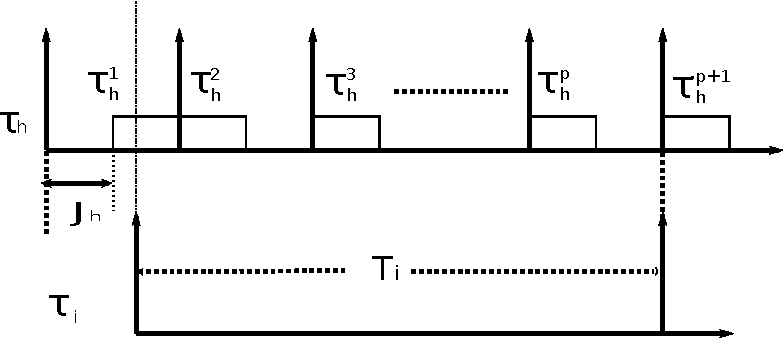
\includegraphics[scale=0.5]{figures/figure18}
\par\end{centering}
\caption{\label{fig17}$\tau_h^p$ has a higher priority than $\tau_i^x$}
\end{figure}

\subsection{Schedulability comparison of G-EDF/LCM and ECM}
\label{performance g-edf-lcm}
We now compare the schedulability of G-EDF/LCM with ECM~\cite{stmconcurrencycontrol:emsoft11} %(FMLP and OMLPprotocols~\cite{key-4,brandenburg2008comparison,key-3}), 
to understand when G-EDF/LCM will perform better. 
Toward this, we compare the total utilization of ECM against that of G-EDF/LCM. In each method, we inflate the $c_i$ for each $\tau_i$ by adding the retry cost suffered by $\tau_i$. Thus, if method $A$ adds retry cost $RC_A(T_i)$ to $c_i$, and method $B$ adds retry cost $RC_B(T_i)$ to $c_i$, then the schedulability of $A$ and $B$ are compared as follows:
\begin{eqnarray}
\sum_{\forall \tau_{i}}\frac{c_{i}+RC_A(T_{i})}{T_{i}} & \le & \sum_{\forall \tau_{i}}\frac{c_{i}+RC_B(T_{i})}{T_{i}}\nonumber\\
\sum_{\forall \tau_{i}}\frac{RC_A(T_{i})}{T_{i}} & \le & \sum_{\forall \tau_{i}}\frac{RC_B(T_{i})}{T_{i}}
\label{eqa}\end{eqnarray}
Thus, schedulability is compared by substituting the retry cost added by synchronization methods in (\ref{eqa}).

\begin{clm}\label{lcm versus ecm}
Let $s_{max}$ be the maximum length atomic section accessing any object $\theta$. Let $\alpha_{max}$ and $\alpha_{min}$ be the maximum and minimum values of $\alpha$ corresponding to $\psi$ for any two atomic sections.  Schedulability of G-EDF/LCM is equal or better than that of  ECM if for any task $\tau_i$:
\begin{equation}
\frac{1-\alpha_{min}}{1-\alpha_{max}} \le \sum_{\forall \tau_h \in \gamma_i}\left\lceil\frac{T_i}{T_h}\right\rceil
\label{edf-lcm-ecm}\end{equation}
\end{clm}
\begin{proof}
Under ECM, $RC(T_{i})$ is upper bounded by:
\begin{equation}
RC(T_{i})\le\sum_{\forall \tau_{h}\in\gamma_{i}}\sum_{\forall \theta\in\ (\theta_{i}\wedge\theta_{h})}\left(\left\lceil\frac{T_{i}}{T_{h}}\right\rceil\sum_{\forall s_{h}^{z}(\theta)}2len(s_{max})\right)\label{eq61}\end{equation}
with the assumption that all lengths of atomic sections of (4) and (8) in~\cite{stmconcurrencycontrol:emsoft11} and~(\ref{eq78}) are replaced by $s_{max}$.
%~\cite{stmconcurrencycontrol:emsoft11}. 
If $\alpha_{max}^{hl}$ in~(\ref{eq78}) is replaced with $\alpha_{max}$, and $\alpha_{min}^{iy}$ in~(\ref{eq78}) is replaced with $\alpha_{min}$. As $\alpha_{max}$, $\alpha_{min}$, and $len(s_{max})$ are all constants, then (\ref{eq78}) is upper bounded by:
\begin{eqnarray}
RC(T_i) & \le & \Bigg(\sum_{\forall \tau_h \in \gamma_i}\sum_{\forall\theta \in \theta_i \wedge \theta_h}\Bigg(\left\lceil\frac{T_{i}}{T_{h}}\right\rceil\sum_{\forall s_{h}^{l}(\theta)}\left(1+\alpha_{max}\right)\nonumber\\
& & len\Big(s_{max}\Big)\Bigg)\Bigg)
 +  \sum_{\forall s_{i}^{y}(\theta)}\Big(1-\alpha_{min}\Big)len\Big(s_{max}\Big)\nonumber\\ 
\label{eq101}\end{eqnarray}
%
If $\beta_1^{ih}$ is the total number of times any instance of $\tau_h$ accesses shared objects with $\tau_i$, then $\beta_1^{ih}=\sum_{\forall \theta\in(\theta_{i}\wedge\theta_{h})}\sum_{\forall s_{h}^{z}(\theta)}$. And if $\beta_2^i$ is the total number of times any instance of $\tau_i$ accesses shared objects with any other instance,   $\beta_2^i=\sum_{\forall s_{i}^{y}(\theta)}$\textit{, where $\theta$ is shared with another task}. Then $\beta_{i}=max\{max_{\forall \tau_h \in \gamma_i}\{\beta_1^{ih}\},\beta_2^i\}$ is the maximum number of accesses to all shared objects by any instance of $\tau_{i}$ or $\tau_{h}$. 
Thus, (\ref{eq61}) becomes:
\begin{equation}
RC(T_{i})\le\sum_{\tau_{h}\in\gamma_{i}}2\left\lceil\frac{T_{i}}{T_{h}}\right\rceil\beta_{i}len(s_{max})
\label{eq63}\end{equation}
and (\ref{eq101}) becomes:
\begin{eqnarray}
RC(T_{i}) & \le & \beta_{i}len(s_{max}) \Bigg((1-\alpha_{min})\nonumber\\
& + & \sum_{\forall \tau_h \in \gamma_i}\left\lceil\frac{T_{i}}{T_{h}}\right\rceil(1+\alpha_{max})\Bigg)
\label{eq102}\end{eqnarray}

We can now compare the total utilization of G-EDF/LCM with that of ECM by comparing~(\ref{eq101}) and~(\ref{eq102}) for all $\tau_i$:
\begin{eqnarray}
& & \sum_{\forall \tau_{i}}\frac{(1-\alpha_{min})+\sum_{\forall \tau_{h}\in\gamma_{i}}\left(\left\lceil\frac{T_{i}}{T_{h}}\right\rceil(1+\alpha_{max})\right)}{T_{i}} \nonumber\\
& \le &   \sum_{\forall \tau_{i}}\frac{\sum_{\forall \tau_{h}\in\gamma_{i}}2\left\lceil\frac{T_{i}}{T_{h}}\right\rceil}{T_{i}}\label{eqc}\end{eqnarray}

(\ref{eqc}) is satisfied if for each $\tau_{i}$ the following condition is satisfied:
\begin{equation*}
(1-\alpha_{min})+\sum_{\forall \tau_h \in \gamma_i}\left(\left\lceil\frac{T_{i}}{T_{h}}\right\rceil(1+\alpha_{max})\right)  \le  2\sum_{\forall \tau_h \in \gamma_i}\left\lceil\frac{T_{i}}{T_{h}}\right\rceil
\end{equation*}
\begin{equation*}
\therefore\frac{1-\alpha_{min}}{1-\alpha_{max}}  \le  \sum_{\forall \tau_h \in \gamma_i}\left\lceil\frac{T_{i}}{T_{h}}\right\rceil
\end{equation*}
Claim follows.
\end{proof}

\subsection{G-EDF/LCM versus lock-free synchronization}
\label{gedf-lcm-lock-free}
We consider the retry-loop lock-free synchronization for G-EDF system in~\cite{key-5}. This lock-free approach is the most relevant to our work. In the following Claim, $s_{max}$ is used to denote $len(s_{max})$.

\begin{clm}
If $r_{max}$ is the maximum execution cost of a single iteration of any retry loop of any task in the retry-loop lock-free algorithm in~\cite{key-5}, and if the upper bound on $s_{max}/r_{max}$ provided by G-EDF/LCM ranges between 0.5 and 2 (which is higher than that provided by ECM), then G-EDF/LCM achieves higher schedulability than retry-loop lock-free approach.
%~\cite{stmconcurrencycontrol:emsoft11}. In some cases, G-EDF/LCM can even provide higher $s_{max}$ than $r_{max}$.
\end{clm}
%
\begin{proof}
From~\cite{key-5}, the retry-loop lock-free algorithm is upper bounded by:
\begin{equation}
RL(T_i)=\sum_{\tau_{h}\in\gamma_{i}}\left(\left\lceil\frac{T_{i}}{T_{h}}\right\rceil +1\right)\beta_{i}r_{max}
\label{eq32}\end{equation}
where $\beta_i$ is as defined in Claim~\ref{lcm versus ecm}.
The retry cost of $\tau_i$ in G-EDF/LCM is upper bounded by (\ref{eq102}). By comparing G-EDF/LCM's total utilization with that of the retry-loop lock-free algorithm, we get:
\begin{eqnarray*}
%& 
& \sum_{\forall \tau_{i}}\frac{\left((1-\alpha_{min})+\sum_{\forall \tau_{h}\in\gamma_{i}}\left(\left\lceil\frac{T_{i}}{T_{h}}\right\rceil(1+\alpha_{max})\right)\right)\beta_{i}s_{max}}{T_{i}}\\
%& 
\le & \sum_{\forall \tau_{i}}\frac{\sum_{\forall \tau_{h}\in\gamma_{i}}\left(\left\lceil\frac{T_{i}}{T_{h}}\right\rceil+1\right)\beta_{i}r_{max}}{T_{i}}\end{eqnarray*}
%
\begin{eqnarray}
\therefore\frac{s_{max}}{r_{max}}\le \frac{\sum_{\forall \tau_{i}}\frac{\sum_{\forall \tau_{h}\in\gamma_{i}}\left(\left\lceil\frac{T_{i}}{T_{h}}\right\rceil+1\right)\beta_{i}}{T_{i}}}{\sum_{\forall \tau_{i}}\frac{\left((1-\alpha_{min})+\sum_{\forall \tau_{h}\in\gamma_{i}}\left(\left\lceil\frac{T_{i}}{T_{h}}\right\rceil(1+\alpha_{max})\right)\right)\beta_{i}}{T_{i}}}
\label{u-gedf-lcm-ecm}\end{eqnarray}

If
\begin{eqnarray}
\frac{s_{max}}{r_{max}}\le \frac{{\sum_{\forall \tau_{h}\in\gamma_{i}}\left(\left\lceil\frac{T_{i}}{T_{h}}\right\rceil+1\right)}}{{(1-\alpha_{min})+\sum_{\forall \tau_{h}\in\gamma_{i}}\left(\left\lceil\frac{T_{i}}{T_{h}}\right\rceil(1+\alpha_{max})\right)}}
\label{t-gedf-lcm-ecm}\end{eqnarray}
for each $\tau_i$, then~(\ref{u-gedf-lcm-ecm}) holds.

Let the number of tasks that have shared objects with $\tau_i$ be $\omega$ (i.e., $\sum_{\tau_h \in \gamma_i}=\omega \ge 1$ since at least one task has a shared object with $\tau_i$, otherwise, there is no conflict between tasks), and let the total number of tasks be $n$, so $1\le \omega \le n-1$, and $\left\lceil\frac{T_i}{T_h}\right\rceil \in [1,\infty[$. To find the minimum and upper values for the upper bound on $s_{max}/r_{max}$, we consider the following cases:-
\begin{itemize}
\item $\alpha_{min} \rightarrow 0, \alpha_{max} \rightarrow 0$
\end{itemize}
$\therefore$~(\ref{t-gedf-lcm-ecm}) will be
\begin{eqnarray}
\frac{s_{max}}{r_{max}} & \le & \frac{{\sum_{\forall \tau_{h}\in\gamma_{i}}\left(\left\lceil\frac{T_{i}}{T_{h}}\right\rceil+1\right)}}{{1+\sum_{\forall \tau_{h}\in\gamma_{i}}\left\lceil\frac{T_{i}}{T_{h}}\right\rceil}}
 =  1+\frac{\omega-1}{1+\sum_{\forall \tau_h \in \gamma_i}\left\lceil\frac{T_i}{T_h}\right\rceil}\nonumber\\
\label{s-r-1}\end{eqnarray}
By substituting edge values for $\omega$ and $\left\lceil\frac{T_i}{T_h}\right\rceil$ into~(\ref{s-r-1}), then the upper bound on $s_{max}/r_{max}$ lies between 1 and 2.

\begin{itemize}
\item $\alpha_{min} \rightarrow 0, \alpha_{max} \rightarrow 1$
\end{itemize}
(\ref{t-gedf-lcm-ecm}) becomes
\begin{eqnarray}
\frac{s_{max}}{r_{max}} & \le & 0.5+ \frac{\omega - 0.5}{1+\sum_{\forall \tau_h \in \gamma_i}\left\lceil\frac{T_i}{T_h}\right\rceil}
\label{s-r-2}\end{eqnarray}
By applying edge values for $\omega$ and $\left\lceil\frac{T_i}{T_h}\right\rceil$ in~(\ref{s-r-2}), then the upper bound on $s_{max}/r_{max}$ lies between 0.5 and 1.5.

\begin{itemize}
\item $\alpha_{min} \rightarrow 1, \alpha_{max} \rightarrow 0$
\end{itemize}
This case is rejected since $\alpha_{min} \le \alpha_{max}$

\begin{itemize}
\item $\alpha_{min} \rightarrow 1, \alpha_{max} \rightarrow 1$
\end{itemize}
$\therefore$~(\ref{t-gedf-lcm-ecm}) becomes
\begin{eqnarray}
\frac{s_{max}}{r_{max}}& \le & \frac{\omega+\sum_{\forall \tau_h \in \gamma_i}\left\lceil\frac{T_i}{T_h}\right\rceil}{2\sum_{\forall \tau_h \in \gamma_i}\left\lceil\frac{T_i}{T_h}\right\rceil} = \frac{\omega}{2\sum_{\forall \tau_h \in \gamma_i}\left\lceil\frac{T_i}{T_h}\right\rceil}+0.5\nonumber\\
\label{s-r-4}\end{eqnarray}
By applying edge values for $\omega$ and $\left\lceil\frac{T_i}{T_h}\right\rceil$ in~(\ref{s-r-4}), then the upper bound on $s_{max}/r_{max}$ lies between 0.5 and 1, which is similar to that achieved by ECM.

So, from the previous cases, the upper bound on $s_{max}/r_{max}$ lies between 0.5 and 2, while in case of ECM~\cite{stmconcurrencycontrol:emsoft11}, it lies between 0.5 and 1. Claim follows.
\end{proof}

\subsection{Response time of G-RMA/LCM}
\label{rma}

\begin{clm}\label{response g-rma/lcm}
Let $\lambda_{2}(j,\theta)=\sum_{\forall s_{j}^{l}(\theta)}len(s_{j}^{l}(\theta))+\alpha_{max}^{jl}len(s_{max}^{j}(\theta))$ where $\alpha_{max}^{jl}$ is the $\alpha$ value corresponding to $\psi$ due to interference of $s_{max}^j(\theta)$ by $s_j^l(\theta)$. The retry cost of any task $\tau_i$ under G-RMA/LCM for $T_i$ is given by:
\begin{eqnarray}
RC\left(T_i\right) & = &
  \sum_{\forall \tau_{j}^{*}}\left(\sum_{\theta\in(\theta_{i}\wedge\theta_{j})}\left(\left(\left\lceil\frac{T_i}{T_{j}}\right\rceil +1\right)\lambda_{2}(j,\theta)\right)\right)\nonumber\\
& + & \sum_{\forall s_{i}^{y}(\theta)}\Big(1-\alpha_{min}^{iy}\Big)len\Big(s_{min}^i(\theta)\Big)
\label{eq60}
\end{eqnarray}
where $\tau_{j}^{*}=\{\tau_{j}|(\tau_{j}\in\gamma_{i})\wedge(p_{j}>p_{i})\}$.
\end{clm}
\begin{proof}
Under G-RMA, all instances of a higher priority task, $\tau_{j}$, can conflict with a lower priority task,
$\tau_{i}$, during $T_{i}$.~(\ref{eq47}) will be used to determine the contribution of each conflicting atomic section in $\tau_j$ to $\tau_i$. Meanwhile, all instances of any task with lower priority than $\tau_{i}$, can conflict with $\tau_i$ during $T_{i}$, and Claims~\ref{LCM_lower_rc} and~\ref{priority_inversion} will be used to determine the contribution of conflicting atomic sections in lower priority tasks to $\tau_i$.
%
  %over the whole $t(T_i)$ (unlike the case of G-EDF/LCM, where (\ref{eq59}) chooses which equation to use depending on whether or not $L$ is less than $\left\lfloor\frac{t(T_{i})-c_{h}}{t(T_{h})}\right\rfloor t(T_{h})+c_{h}$).
Using the previous notations and Claim 3 in~\cite{stmconcurrencycontrol:emsoft11}, Claim follows.
\end{proof}

The response time is calculated by (17) in~\cite{stmconcurrencycontrol:emsoft11} with replacing $RC(R_i^{up})$ with $RC(T_i)$.

\subsection{Schedulability Comparison of G-RMA/LCM with RCM}
\label{rma eval}

\begin{clm}
Under the same assumptions of Claims~\ref{lcm versus ecm} and~\ref{response g-rma/lcm}, G-RMA/LCM's schedulability is equal or better than that of RCM if:
\begin{equation}
\frac{1-\alpha_{min}}{1-\alpha_{max}}\le \sum_{\forall \tau_j^*}\left( \left\lceil\frac{T_i}{T_j}\right\rceil +1 \right)
\label{eq70}\end{equation}
\end{clm}
%
\begin{proof}
Under the same assumptions as that of Claims~\ref{lcm versus ecm} and~\ref{response g-rma/lcm}, (\ref{eq60}) can be upper bounded as:
\begin{eqnarray}
RC(T_i) & \le & \sum_{\forall \tau_{j}^{*}}\bigg(\left(\left\lceil\frac{T_{i}}{T_{j}}\right\rceil +1\right)(1+\alpha_{max})
 len(s_{max})\beta_{i}\bigg)\nonumber\\
 & + & (1-\alpha_{min})len(s_{max})\beta_{i}\label{eq68}\end{eqnarray}
 
For RCM, (16) in~\cite{stmconcurrencycontrol:emsoft11} for $RC(T_{i})$ is upper bounded by:
\begin{equation*}
RC(T_{i})\le\sum_{\forall \tau_{j}^{*}}\left(\left\lceil\frac{T_{i}}{T_{j}}\right\rceil +1\right)2\beta_{i}len(s_{max})\label{eq69}\end{equation*}\
By comparing the total utilization of G-RMA/LCM with that of RCM,
we get:
\begin{eqnarray}
 & \sum_{\forall\tau_{i}}\frac{len\left(s_{max}\right)\beta_{i}\left(\left(1-\alpha_{min}\right)+\sum_{\forall\tau_{j}^{*}}\left(\left(\left\lceil\frac{T_{i}}{T_{j}}\right\rceil+1\right)\left(1+\alpha_{max}\right)\right)\right)}{T_{i}}\nonumber\\
\le & \sum_{\forall\tau_{i}}\frac{2len\left(s_{max}\right)\beta_{i}\sum_{\forall\tau_{j}^{*}}\left(\left\lceil\frac{T_{i}}{T_{j}}\right\rceil+1\right)}{T_{i}}\label{grma-lcm-rcm}\end{eqnarray}
(\ref{grma-lcm-rcm}) is satisfied if $\forall \tau_i$~(\ref{eq70}) is satisfied. Claim follows.
\end{proof}

\section{Conclusions}
\label{sec:conclusions}

In ECM and RCM, a task incurs at most $2s_{max}$ retry cost for each one of its atomic sections due to conflict
with another task's atomic section. With LCM, this retry cost is reduced to $(1+\alpha_{max})s_{max}$ for each aborted atomic section. In ECM and RCM, tasks do not retry due to lower priority tasks, while in LCM, this happens. In G-EDF/LCM, retrial due to lower priority job is encountered only from a task $\tau_{j}$'s last instance during $\tau_{i}$'s period. This is not the case with G-RMA/LCM, because,  each higher priority task can be aborted and retried by any instance of lower priority tasks. Schedulability of G-EDF/LCM and G-RMA/LCM can be better or equal to ECM and RCM, respectively, by proper choices for $\alpha_{min}$ and $\alpha_{max}$. Schedulability of G-EDF/LCM is better than retry-loop lock-free approach for G-EDF system if the upper bound on $s_{max}/r_{max}$ lies between 0.5 and 2, which is higher than that achieved by ECM.

Our work has only further scratched the surface of real-time STM. Our work is analytical, because our question is analytical---i.e., how to increase STM's schedulability advantage through a novel CM design? That said, significant insights can be gained by experimental work, which is outside this work's  scope. For e.g., what are the typical range of values for the different parameters that affect the retry and blocking costs (and hence response time)? How tight is our derived upper bounds in practice? 
What is the most practically suitable
value for $\psi$, $\alpha_{min}$, and $\alpha_{max}$? Is it more suitable to have different $\psi$s for different atomic section lengths, instead of using a common one? Future work is expected to include multiple objects per atomic section and nested atomic sections.


%\bibliographystyle{acmsmall}
%\bibliography{global_bibliography}

\bibliographystyle{abbrv}
\bibliography{global_bibliography}

\end{document}
